\documentclass[tikz,border=6pt]{standalone}

\usepackage{amsmath}
\usetikzlibrary{arrows.meta,calc}

\definecolor{panelbg}{HTML}{E8EEF3}
\definecolor{panelborder}{HTML}{666666}

\definecolor{bluec}{HTML}{4169A9}
\definecolor{purplec}{HTML}{8A2E99}
\definecolor{orangec}{HTML}{D97A00}
\definecolor{greenc}{HTML}{3D8B35}
\definecolor{redc}{HTML}{C83232}

\tikzset{
    point/.style={
        circle,
        draw=#1!70!black,
        fill=#1!75,
        line width=0.2pt,
        minimum size=2.5pt,
        inner sep=0pt
    },
    bigpoint/.style={
        circle,
        draw=#1!70!black,
        fill=#1!72,
        line width=0.5pt,
        minimum size=10pt,
        inner sep=0pt
    },
    legendpoint/.style={
        circle,
        draw=#1!70!black,
        fill=#1!72,
        line width=0.3pt,
        minimum size=6pt,
        inner sep=0pt
    },
    cluster/.style={
        draw=#1!70!black,
        fill=#1!12,
        dashed,
        line width=0.8pt
    },
    islandlink/.style={
        <->,
        >=Latex,
        dashed,
        line width=0.55pt,
        draw=black!55,
        opacity=0.70,
        line cap=round
    },
    legendtitle/.style={
        font=\bfseries\Large,
        align=center
    },
    legendtext/.style={
        font=\normalsize,
        align=center
    }
}

\begin{document}

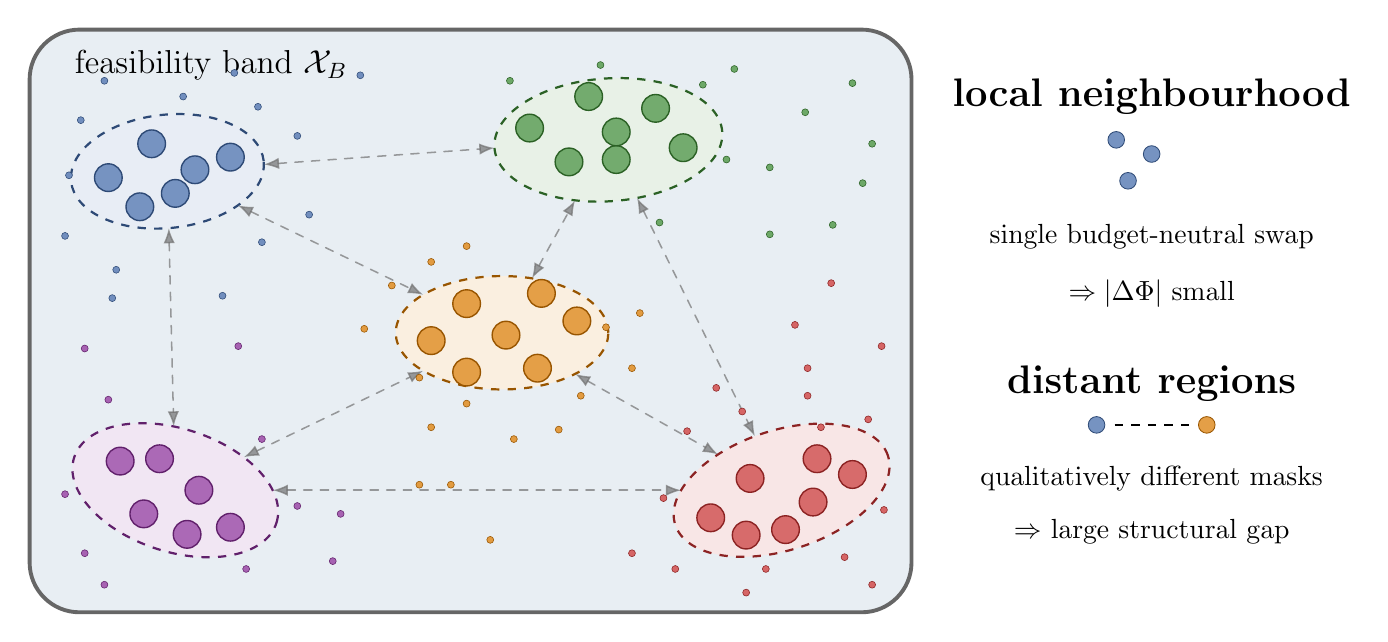
\begin{tikzpicture}[font=\sffamily]

% =================================================
% Main feasibility panel
% =================================================
\draw[
    rounded corners=18pt,
    fill=panelbg,
    draw=panelborder,
    line width=1.4pt
]
(0,0) rectangle (11.2,7.4);

\node[anchor=west, font=\large] at (0.45,6.95)
{feasibility band $\mathcal{X}_{B}$};

% =================================================
% Cluster ellipses
% =================================================
\draw[cluster=bluec, rotate around={6:(1.75,5.6)}]
(1.75,5.6) ellipse (1.23 and 0.72);

\draw[cluster=purplec, rotate around={-18:(1.85,1.55)}]
(1.85,1.55) ellipse (1.35 and 0.78);

\draw[cluster=orangec, rotate around={0:(6.0,3.55)}]
(6.0,3.55) ellipse (1.35 and 0.72);

\draw[cluster=greenc, rotate around={4:(7.35,6.0)}]
(7.35,6.0) ellipse (1.45 and 0.78);

\draw[cluster=redc, rotate around={18:(9.55,1.55)}]
(9.55,1.55) ellipse (1.42 and 0.76);


% =================================================
% Exact bidirectional arrows between selected island pairs
% =================================================
% For an island ellipse with centre c, radii (a,b), rotation theta,
% and direction unit vector u from island i to island j:
%
%   p_boundary = c + t u
%
% where
%
%   t = 1 / sqrt((u'_x/a)^2 + (u'_y/b)^2),
%   u' = R(-theta) u.
%
% Therefore every arrow starts and ends on the actual ellipse boundary,
% not on hand-picked coordinates.
%
% To reduce visual clutter, the two far links blue<->red and purple<->green
% are omitted. Their relation is represented transitively through neighbouring islands.
%
% blue-purple: start=(1.7678,4.8787), end=(1.8300,2.3601), gap=2.5193
% blue-orange: start=(2.6453,5.1682), end=(4.9988,4.0330), gap=2.6129
% blue-green: start=(2.9756,5.6875), end=(5.9037,5.8967), gap=2.9356
% removed for clarity: blue-red: start=(2.6177,5.1494), end=(8.7126,1.9848), gap=6.8674
% purple-orange: start=(2.7201,1.9693), end=(4.9984,3.0673), gap=2.5290
% removed for clarity: purple-green: start=(2.5270,2.0978), end=(6.5114,5.3215), gap=5.1252
% purple-red: start=(3.0873,1.5500), end=(8.2737,1.5500), gap=5.1865
% orange-green: start=(6.3806,4.2408), end=(6.9267,5.2318), gap=1.1315
% orange-red: start=(6.9281,3.0271), end=(8.7429,2.0047), gap=2.0830
% green-red: start=(7.7149,5.2620), end=(9.2106,2.2364), gap=3.3751
\draw[islandlink] (1.7678,4.8787) -- (1.8300,2.3601);
\draw[islandlink] (2.6453,5.1682) -- (4.9988,4.0330);
\draw[islandlink] (2.9756,5.6875) -- (5.9037,5.8967);
\draw[islandlink] (2.7201,1.9693) -- (4.9984,3.0673);
\draw[islandlink] (3.0873,1.5500) -- (8.2737,1.5500);
\draw[islandlink] (6.3806,4.2408) -- (6.9267,5.2318);
\draw[islandlink] (6.9281,3.0271) -- (8.7429,2.0047);
\draw[islandlink] (7.7149,5.2620) -- (9.2106,2.2364);

% =================================================
% Big cluster points
% =================================================
% Blue
\foreach \p in {
    (1.00,5.52),(1.55,5.95),(2.10,5.62),
    (2.55,5.78),(1.85,5.32),(1.4,5.15)
}{
    \node[bigpoint=bluec] at \p {};
}

% Purple
\foreach \p in {
    (1.15,1.92),(1.65,1.95),(2.15,1.55),
    (1.45,1.25),(2.55,1.08),(2.0,0.99)
}{
    \node[bigpoint=purplec] at \p {};
}

% Orange
\foreach \p in {
    (5.10,3.45),(5.55,3.92),(6.05,3.52),
    (6.50,4.05),(6.95,3.70),(5.55,3.05),
    (6.45,3.10)
}{
    \node[bigpoint=orangec] at \p {};
}

% Green
\foreach \p in {
    (6.35,6.15),(7.10,6.55),(7.45,5.75),
    (7.95,6.40),(8.30,5.90),(6.85,5.72),
    (7.45,6.10)
}{
    \node[bigpoint=greenc] at \p {};
}

% Red
\foreach \p in {
    (8.65,1.20),(9.15,1.70),(9.60,1.05),
    (10.00,1.95),(10.45,1.75),(9.95,1.40),
    (9.10,0.98)
}{
    \node[bigpoint=redc] at \p {};
}

% =================================================
% Small background points
% All small points are assigned by nearest cluster centre:
% color(p) = argmin_c sqrt((x_p - x_c)^2 + (y_p - y_c)^2)
%
% Cluster centres:
% blue   = (1.75, 5.60)
% purple = (1.85, 1.55)
% orange = (6.00, 3.55)
% green  = (7.35, 6.00)
% red    = (9.55, 1.55)
%
% Ambiguous boundary points with tiny nearest-vs-runner-up margins
% were removed so that the visual colour matches the nearest region.
% =================================================
\foreach \p in {
    (2.60,6.85),(4.20,6.82),(0.95,6.75),(1.95,6.55),
    (2.90,6.42),(0.65,6.25),(3.40,6.05),(0.50,5.55),
    (3.55,5.05),(0.45,4.78),(2.95,4.70),(1.10,4.35),
    (2.45,4.02),(1.05,3.99)
}{
    \node[point=bluec] at \p {};
}

\foreach \p in {
    (2.65,3.38),(0.70,3.35),(1.00,2.70),(2.95,2.20),
    (0.45,1.50),(3.40,1.35),(3.95,1.25),(0.70,0.75),
    (3.85,0.65),(2.75,0.55),(0.95,0.35)
}{
    \node[point=purplec] at \p {};
}

\foreach \p in {
    (5.55,4.65),(5.10,4.45),(4.60,4.15),(7.75,3.80),
    (7.32,3.62),(4.25,3.60),(7.65,3.10),(4.95,2.98),
    (7.00,2.75),(5.55,2.65),(5.10,2.35),(6.72,2.32),
    (6.15,2.20),(4.95,1.62),(5.35,1.62),(5.85,0.92)
}{
    \node[point=orangec] at \p {};
}

\foreach \p in {
    (7.25,6.95),(8.95,6.90),(6.10,6.75),(10.45,6.72),
    (8.55,6.70),(9.85,6.35),(10.70,5.95),(8.85,5.75),
    (9.40,5.65),(10.58,5.45),(8.00,4.95),(10.20,4.92),
    (9.40,4.80)
}{
    \node[point=greenc] at \p {};
}

\foreach \p in {
    (10.18,4.18),(9.72,3.65),(10.82,3.38),(9.88,3.10),
    (8.72,2.85),(9.88,2.75),(9.05,2.55),(10.65,2.45),
    (10.05,2.35),(8.35,2.30),(8.05,1.45),(10.85,1.30),
    (7.65,0.75),(10.35,0.70),(8.20,0.55),(9.35,0.55),
    (10.70,0.35),(9.10,0.25)
}{
    \node[point=redc] at \p {};
}

% =================================================
% Legend (moved right, smaller circles, more spacing)
% =================================================
\node[legendtitle, anchor=north] at (14.25,6.90)
{local neighbourhood};

\node[legendpoint=bluec] at (13.80,6.00) {};
\node[legendpoint=bluec] at (14.25,5.82) {};
\node[legendpoint=bluec] at (13.95,5.48) {};

\node[legendtext, anchor=north] at (14.25,5.05)
{single budget-neutral swap};

\node[legendtext, anchor=north] at (14.25,4.35)
{$\Rightarrow |\Delta \Phi|$ small};

\node[legendtitle, anchor=north] at (14.25,3.25)
{distant regions};

\node[legendpoint=bluec]   at (13.55,2.38) {};
\node[legendpoint=orangec] at (14.95,2.38) {};
\draw[dashed, line width=0.8pt] (13.78,2.38) -- (14.72,2.38);

\node[legendtext, anchor=north] at (14.25,1.98)
{qualitatively different masks};

\node[legendtext, anchor=north] at (14.25,1.30)
{$\Rightarrow$ large structural gap};

\end{tikzpicture}

\end{document}